\subsection{极大环面}

设 G 是李群。G 的环面是指 G 的一个闭子群，它本身是一个环面（§1 第 2 节），换言之即任一交换的连通紧子群。G 的环面所成的集按包含关系排序后，其极大元称为 G 的极大环面。

定理 2. 设 G 是连通紧李群。

\begin{enumerate}
\def\labelenumi{\alph{enumi})}
\item
  \(\mathbf{G}\) 的诸极大环面的李代数是 \(\mathrm{L}(\mathrm{G})\) 的嘉当子代数。
\item
  设 \(\mathrm{T}_1\) 与 \(\mathrm{T}_2\) 是 \(\mathbf{G}\) 的两个极大环面。则存在 \(g \in \mathbf{G}\) 使得 \(\mathrm{T}_2 = g\mathrm{T}_1g^{-1}\) 。
\item
  G 是它的诸极大环面之并。
\end{enumerate}

设 t 是 L(G) 的一个嘉当子代数；G 中以 t 为李代数的积分子群是闭的（第 VII 章，§2，第 1 节，命题 4 的推论 4）且交换的（定理 1），因而是 G 的一个环面。若 T 是 G 的极大环面，则其李代数交换，故包含于 L(G) 的某个嘉当子代数（定理 1）。由此可知，G 的极大环面恰是 L(G) 的嘉当子代数所对应的 G 的积分子群，由此得 a)。断言 b) 由定理 1 得出，因为典则同态 G → Int(L(G)) 是满射（第 III 章，§6，第 4 节，命题 10 的推论 4）。

用 X 表示 G 的诸极大环面之并，设 T 是 G 的一个极大环面。连续映射 \((g,t)\mapsto gtg^{-1}\) （从 \(G\times T\) 到 G）的像是 X，因而 X 在 G 中闭；于是，为证 c)，只需证明 X 在 G 中开；由于 X 在内自同构下不变，只需证明对一切 \(a \in \mathrm{T}\) ， \(\mathrm{X}\) 是 \(a\) 的邻域。我们对 \(\mathrm{G}\) 的维数作归纳，并区分两种情形：

\begin{enumerate}
\def\labelenumi{\arabic{enumi})}
\item
  a 不是 G 的中心元。设 H 是 a 在 G 中的中心化子的单位元连通分支；这是 G 的一个异于 G 的连通紧子群，它包含 T，因而包含 a。由于 Ad a 半单（ \(\S1\) ，第 1 节），H 的李代数是 Ad a - 1 的幂零空间；于是由第 VII 章 \(\S4\) 第 2 节命题 4，H 的诸共轭之并 Y 是 a 的邻域。由归纳假设，\(H \subset X\) ，故 \(Y \subset X\) ；从而 X 是 a 的邻域。
\item
  a 是 G 的中心元。只需证明对 L(G) 中一切 x，\(a \exp x\) 属于 X。而 L(G) 的每个元素 x 都属于 G 的某个嘉当子代数（定理 1）；对应的积分子群 T' 包含 \(\exp x\) ；由于它共轭于 T，它包含 a，因而包含 \(a \exp x\) ，此即所要证明的。
\end{enumerate}

推论 1. a) \(\mathbf{G}\) 的指数映射是满射。

\begin{enumerate}
\def\labelenumi{\alph{enumi})}
\setcounter{enumi}{1}
\tightlist
\item
  对一切 \(n \geq 1\) ，映射 \(g \mapsto g^n\) 从 \(\mathbf{G}\) 到其自身是满射。
\end{enumerate}

事实上，\(\exp(\mathrm{L}(\mathrm{G}))\) 包含 G 的所有极大环面，由此得 a)。断言

\begin{enumerate}
\def\labelenumi{\alph{enumi})}
\setcounter{enumi}{1}
\tightlist
\item
  由公式 \((\exp x)^n = \exp nx\)（\(x\) 属于 \(\mathrm{L}(\mathrm{G})\) ）得出。
\end{enumerate}

注 1. 存在紧子集 \(\mathrm{K}\) （含于 \(\mathrm{L}(\mathrm{G})\) ）使得 \(\exp_{\mathrm{G}}(\mathrm{K}) = \mathrm{G}\) 。事实上，若 \(\mathrm{T}\) 是 \(\mathrm{G}\) 的极大环面，则存在紧子集 \(\mathrm{C} \subset \mathrm{L}(\mathrm{T})\) 使得 \(\exp_{\mathrm{T}}(\mathrm{C}) = \mathrm{T}\) ；只需取 \(\mathrm{K} = \bigcup_{g \in \mathrm{G}} (\operatorname{Ad} g)(\mathrm{C})\) 。

推论 2. G 的诸极大环面之交是 G 的中心。

设 x 是 G 的中心的一个元素；由定理 2 c)，存在包含 x 的 G 的极大环面 T；于是 x 属于 T 的所有共轭，从而属于 G 的所有极大环面。反之，若 x 属于 G 的所有极大环面，则由定理 2 c)，x 与 G 的每个元素交换。

推论 3. 设 \(g \in \mathbf{G}\) ，\(\mathbf{C}\) 是它的中心化子。则 \(g\) 属于 \(\mathrm{C}_0\) ；群 \(\mathrm{C}_0\) 是 \(\mathbf{G}\) 的包含 \(g\) 的诸极大环面之并。

存在包含 g 的 G 的极大环面 T（定理 2 c)），它包含于 \(C_{0}\) 。此外，群 \(C_{0}\) 是连通紧李群，因而是它的诸极大环面之并（定理 2 c)）；这些极大环面都包含 g（推论 2），故它们恰是 G 的包含 g 的极大环面。

推论 4. 设 \(g \in G\) 。若 \(g\) 正则（第 VII 章，§4，第 2 节，定义 2），则它属于唯一的极大环面，即其中心化子的单位元连通分支。否则，它属于无穷多个极大环面。

由于 Ad g 半单，Ad g-1 的幂零空间的维数也就是 g 的中心化子 C 的维数。由同前命题 8 与定理 1，g 正则当且仅当 \(C_{0}\) 是 G 的极大环面。结论由推论 3 立即得出。

推论 5. a) 设 S 是 G 的一个环面。S 的中心化子是连通的；它是 G 的包含 S 的诸极大环面之并。

\begin{enumerate}
\def\labelenumi{\alph{enumi})}
\setcounter{enumi}{1}
\tightlist
\item
  设 \(\mathfrak{s}\) 是 \(\mathrm{L}(\mathrm{G})\) 的交换子代数。\(\mathfrak{s}\) 在 \(\mathrm{G}\) 中的固定子群是连通的；它是 \(\mathrm{G}\) 的李代数包含 \(\mathfrak{s}\) 的诸极大环面之并。
\end{enumerate}

为证 \(a\) ，只需证明：若 G 的元素 \(g\) 与 S 交换，则存在 G 的极大环面同时包含 S 与 \(g\) 。设 C 是 \(g\) 的中心化子，则 \(g \in \mathrm{C}_0\) （推论 3）且 \(\mathrm{S} \subset \mathrm{C}_0\) ；若 T 是连通紧李群 \(\mathrm{C}_0\) 的包含 S 的极大环面，则 \(g \in \mathrm{T}\) （推论 2），由此得 \(a\) )。断言 \(b\) ) 由 \(a\) ) 应用于以 \(\mathfrak{s}\) 为李代数的积分子群的闭包得出，依据是第 III 章，§9，第 3 节，命题 9。

\pandocbounded{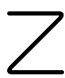
\includegraphics[keepaspectratio]{images/part002_b9f4d066.jpg}}

注 2. 由推论 5 可知，G 的极大环面是极大交换子群。逆命题不真：例如在群 \(\mathbf{SO}(3,\mathbf{R})\) 中，极大环面都是 1 维的，因而不能包含同构于 \((\mathbf{Z}/2\mathbf{Z})^{2}\) 的对角矩阵组成的子群。此外，若 \(g \in \mathbf{SO}(3,\mathbf{R})\) 是非纯量对角矩阵，则 g 是 \(\mathbf{SO}(3,\mathbf{R})\) 的正则元，其中心化子不连通（参见推论 4）。

推论 6. G 的极大环面是自身的中心化子，并且是其李代数的固定子群。

设 T 是 G 的极大环面，C 是它的中心化子；由于 \(L(T)\) 是 \(L(G)\) 的嘉当子代数，我们有 \(L(T) = L(C)\) ，又因 C 连通（推论 5），故 C = T。

推论 7. 设 T 与 T' 是 G 的两个极大环面，A 是 T 的子集，s 是把 A 变到 T' 中的 G 的自同构。则存在 \(g \in G\) 使得 \(s \circ (\operatorname{Int} g)\) 把 T 变到 T' 且在 A 上与 s 相合。

设 C 是 A 的中心化子。则 T 与 \(s^{-1}(T')\) 是 \(C_{0}\) 的两个极大环面；\(C_{0}\) 中满足 \((\operatorname{Int} g)(\mathrm{T}) = s^{-1}(\mathrm{T}')\) 的任何元素 g 都具有所要的性质。

推论 8. 设 H 是紧李群，T 是 H 的极大环面。则 \(\mathrm{H} = \mathrm{N}_{\mathrm{H}}(\mathrm{T}) \cdot \mathrm{H}_{0}\) ，且 \(\mathrm{N}_{\mathrm{H}}(\mathrm{T})\) 到 H 中的单射诱导一个从 \(\mathrm{N}_{\mathrm{H}}(\mathrm{T}) / \mathrm{N}_{\mathrm{H}_{0}}(\mathrm{T})\) 到 \(H/H_{0}\) 上的同构。

设 \(h \in H\) 。则 \(h^{-1}Th\) 是 \(H_0\) 的极大环面，故（定理 2）存在 \(g \in H_0\) 使得 \(hg \in N_H(T)\) ；于是 \(h\) 属于 \(N_H(T).H_0\) ，第一个断言得证。第二个断言立即得证。

注。3) 设 G 是李代数为紧李代数的连通李群。G 的嘉当子群是以 L(G) 的嘉当子代数为李代数的积分子群（连通紧群的嘉当子群因此就是它的极大环面）。如果把处处出现的用语「极大环面」换成「嘉当子群」，定理 2 及其诸推论对 G 仍然成立。这立即由下述事实得出：依据 §1 第 4 节命题 5，G 是向量群 V 与连通紧群 K 的直积，且 G 的嘉当子群是 V 与 K 的极大环面之积。此外，注意由上面的推论 6 可知，G 的嘉当子群也可以定义为 L(G) 的嘉当子代数的固定子群。

* 4) 定理 2 的部分 \(c\) 也可按如下方式证明。给 G 装备一个不变黎曼度量（§1 第 3 节，命题 3）。于是，对 G 的任一元素 \(g\) ，存在通过 \(g\) 与 G 的单位元的极大测地线（Hopf-Rinow 定理），并且可以验证这样一条测地线的闭包是 G 的一个子环面。*

